\documentclass[12pt,a4paper]{report}

% --- Encodage et langue ---
\usepackage[utf8]{inputenc}
\usepackage[T1]{fontenc}
\usepackage[french]{babel}

% --- Mise en page et typographie ---
\usepackage[top=2.5cm, bottom=2.5cm, left=2.5cm, right=2.5cm]{geometry}
\usepackage{lmodern}
\usepackage{microtype}
\usepackage{setspace}
\onehalfspacing

% --- Couleurs, tableaux, figures et liens ---
\usepackage{xcolor}
\usepackage{graphicx}
\usepackage{float}
\usepackage{booktabs}
\usepackage{longtable}
\usepackage{array}
\usepackage{tabularx}
\usepackage{fancyhdr}
\usepackage{titlesec}
\usepackage{hyperref}

\definecolor{uaszGreen}{HTML}{1B5E20}
\definecolor{uaszGold}{HTML}{C68B2C}
\definecolor{uaszDark}{HTML}{1E293B}
\definecolor{uaszLight}{HTML}{F4F7F5}

\hypersetup{
    colorlinks=true,
    linkcolor=uaszGreen,
    urlcolor=uaszGold,
    citecolor=uaszGreen,
    pdftitle={Rapport Technique - Plateforme Microservices Patrimoine Touristique de la Casamance},
    pdfauthor={Ibrahima DIALLO, Matar NDOUR}
}

% --- En-têtes et pieds de page ---
\pagestyle{fancy}
\fancyhf{}
\fancyhead[L]{\small\textcolor{uaszDark}{UASZ -- L3 Ingénierie Informatique}}
\fancyhead[R]{\small\textcolor{uaszDark}{Plateforme Patrimoine Touristique de la Casamance}}
\fancyfoot[C]{\thepage}
\renewcommand{\headrulewidth}{0.4pt}

% --- Style des chapitres ---
\titleformat{\chapter}[display]
  {\normalfont\huge\bfseries\color{uaszGreen}}
  {\chaptertitlename\ \thechapter}{14pt}{\Huge\color{uaszDark}}

\begin{document}

% =============================================================================
% PAGE DE GARDE
% =============================================================================
\begin{titlepage}
    \centering
    {\Large\bfseries Université Assane Seck de Ziguinchor (UASZ)\par}
    \vspace{0.3cm}
    {\large UFR Sciences et Technologies -- Département Informatique\par}
    {\normalsize Licence 3 en Ingénierie Informatique\par}
    \vspace{1.2cm}
    \rule{\textwidth}{1.5pt}\\[0.5cm]
    {\Huge\bfseries\color{uaszGreen} Plateforme de Gestion et de Valorisation du Patrimoine Touristique de la Casamance\par}
    \vspace{0.4cm}
    {\Large\color{uaszDark} Rapport Technique d'Architecture Microservices, Sécurité Zero-Trust, Déploiement Docker et Validation Complète\par}
    \rule{\textwidth}{1.5pt}
    \vspace{1.5cm}

    \begin{minipage}[t]{0.48\textwidth}
        \raggedright
        \textbf{Réalisé par :}\\
        \large Ibrahima \textsc{DIALLO}\\
        \large Matar \textsc{NDOUR}
    \end{minipage}
    \hfill
    \begin{minipage}[t]{0.48\textwidth}
        \raggedleft
        \textbf{Enseignant encadrant :}\\
        \large Dr Lamine \textsc{FATY}\\
        \normalsize Développement d'Applications Orientées Services
    \end{minipage}

    \vfill
    {\large Dépôt GitHub : \texttt{https://github.com/ona79/micro-service}\par}
    \vspace{0.3cm}
    {\large Année universitaire 2025 -- 2026\par}
    {\normalsize Ziguinchor, Sénégal -- Novembre 2026\par}
\end{titlepage}

% =============================================================================
% SOMMAIRE, LISTES DES FIGURES ET TABLEAUX
% =============================================================================
\tableofcontents
\listoffigures
\listoftables
\newpage

% =============================================================================
% CHAPITRE 1 : INTRODUCTION ET GESTION DE VERSION
% =============================================================================
\chapter{Introduction et Contexte du Projet}

\section{Objectif de la plateforme}
Dans le cadre du module \emph{Développement d'Applications Orientées Services} à l'Université Assane Seck de Ziguinchor (UASZ), nous avons conçu, développé, sécurisé et validé une plateforme numérique complète dédiée à la gestion et à la valorisation du patrimoine touristique de la Casamance.

Le système repose sur une architecture distribuée orientée microservices respectant les principes du \emph{Database-per-Service}, une sécurité \emph{Zero-Trust} avec contrôle d'accès basé sur les rôles et permissions (RBAC/BOLA), un annuaire de services dynamique (Netflix Eureka) et une interface web moderne sous Angular~22 servie par Nginx.

\section{Collaboration Git et consolidation des branches}
Le développement collaboratif entre \textbf{Ibrahima DIALLO} et \textbf{Matar NDOUR} a été structuré autour de branches thématiques par lots fonctionnels et correctifs (\texttt{feature/p01-*} à \texttt{feature/p07-8-*}, \texttt{fix/*}) sur le dépôt GitHub \texttt{ona79/micro-service}.

Lors de la phase de consolidation finale :
\begin{itemize}
    \item Toutes les branches fonctionnelles ont été intégrées et consolidées sur \texttt{develop}, puis alignées sur \texttt{main} et \texttt{deploy} au commit \texttt{041c989} (89 commits, 22 branches).
    \item La branche \texttt{feature/p07-5-functional-audit} a été fusionnée proprement sans conflit pour intégrer l'ensemble des livrables d'audit fonctionnel.
    \item La branche \texttt{develop} a été conservée comme branche de travail active.
\end{itemize}

\begin{figure}[H]
    \centering
    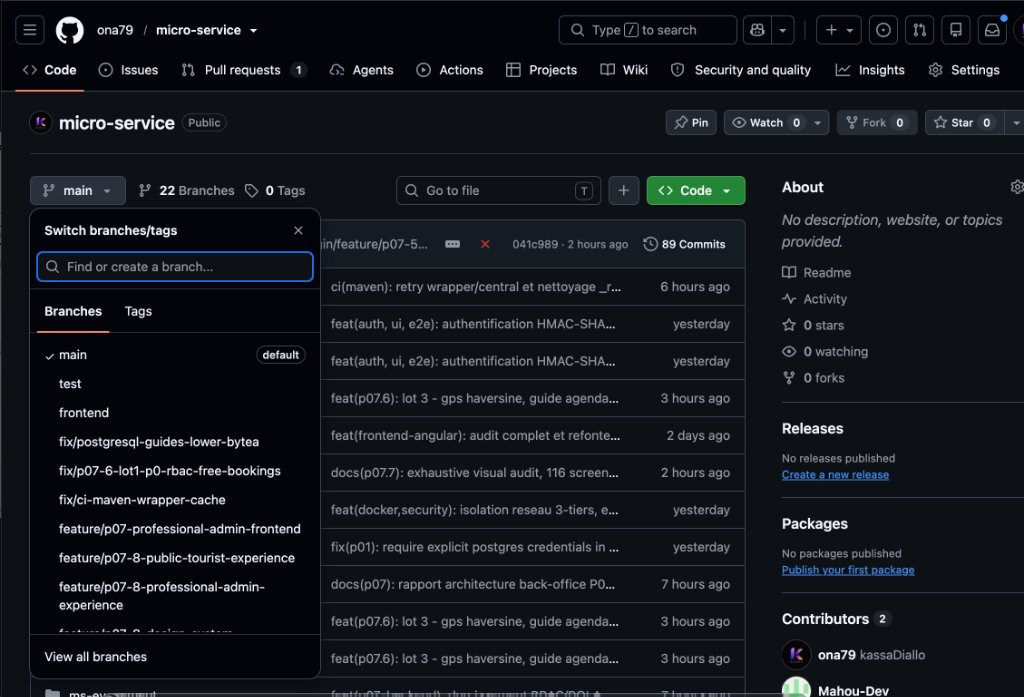
\includegraphics[width=0.92\textwidth]{images/github_branches_contributors.jpg}
    \caption{Preuve de consolidation GitHub sur \texttt{ona79/micro-service} : 22 branches, 89 commits, commit \texttt{041c989} et contributeurs.}
    \label{fig:github-repo}
\end{figure}

% =============================================================================
% CHAPITRE 2 : ARCHITECTURE MICROSERVICES ET INFRASTRUCTURE
% =============================================================================
\chapter{Architecture Microservices et Infrastructure Docker}

\section{Stack technologique}
\begin{itemize}
    \item \textbf{Back-End (9 services Java)} : Java~21 (Temurin/OpenJDK), Spring Boot~4.1.0, Spring Cloud~2025.1.4, Spring Data JPA, MapStruct~1.6.3, Lombok, OpenFeign, Spring Cloud LoadBalancer, Netflix Eureka.
    \item \textbf{Persistance} : PostgreSQL~16 avec 7 bases indépendantes et migrations versionnées Flyway~10 (\texttt{ddl-auto: validate} en profil \texttt{prod}).
    \item \textbf{Front-End} : Angular~22 (Standalone Components, Signals, Router), Leaflet (cartographie OpenStreetMap), QRCode / \texttt{html5-qrcode}, Nginx en reverse proxy (\texttt{/api/**} vers \texttt{api-gateway:8090}).
    \item \textbf{Conteneurisation} : Docker Compose avec isolation réseau en 3 zones (\texttt{edge-net}, \texttt{app-net} interne, \texttt{data-net} interne).
\end{itemize}

\section{Cartographie des services et bases de données}

\begin{table}[H]
\centering
\caption{Cartographie des 11 conteneurs Docker Compose et de leurs responsabilités}
\label{tab:services-mapping}
\small
\begin{tabularx}{\textwidth}{@{}l l l X@{}}
\toprule
\textbf{Service} & \textbf{Port} & \textbf{Base PostgreSQL} & \textbf{Rôle principal} \\
\midrule
\texttt{frontend-angular} & 80 (hôte) & -- & Interface Angular 22 + proxy Nginx \texttt{/api} \\
\texttt{api-gateway} & 8090 (interne) & -- & Point d'entrée unique, validation HMAC et routage \\
\texttt{discovery-server} & 8761 (interne) & -- & Annuaire de services Netflix Eureka \\
\texttt{ms-patrimoine} & 3001 (interne) & \texttt{patrimoine\_db} & Sites patrimoniaux, GPS, capacités \\
\texttt{ms-circuit} & 3002 (interne) & \texttt{circuit\_db} & Circuits touristiques, étapes, affectation guide \\
\texttt{ms-evenement} & 3003 (interne) & \texttt{evenement\_db} & Événements culturels, festivals, jauges \\
\texttt{ms-reservation} & 3004 (interne) & \texttt{reservation\_db} & Réservations, e-billets QR, avis \& modération \\
\texttt{ms-utilisateur} & 3005 (interne) & \texttt{utilisateur\_db} & Comptes, sessions, RBAC 48 permissions, guides \\
\texttt{ms-paiement} & 3006 (interne) & \texttt{paiement\_db} & Paiements simulés, idempotence et Outbox \\
\texttt{ms-notification} & 3007 (interne) & \texttt{notification\_db} & Boîte de réception notifications utilisateur \\
\texttt{postgres} & 5432 (interne) & 7 bases & Serveur PostgreSQL 16 isolé sur \texttt{data-net} \\
\bottomrule
\end{tabularx}
\end{table}

% =============================================================================
% CHAPITRE 3 : SÉCURITÉ ZERO-TRUST ET RBAC
% =============================================================================
\chapter{Sécurité Zero-Trust, Authentification et RBAC}

\section{Authentification par cookie HttpOnly et propagation HMAC}
La sécurité de la plateforme suit une approche \emph{Zero-Trust} :
\begin{itemize}
    \item Les sessions utilisateurs sont signées en \textbf{HMAC-SHA256} (\texttt{SECURITY\_SESSION\_SECRET}, entropie minimale de 256 bits) et stockées dans un cookie \texttt{HttpOnly}.
    \item Les secrets d'exemple (\texttt{CHANGE\_ME}) sont explicitement rejetés au démarrage en profil \texttt{prod}.
    \item La passerelle \texttt{api-gateway} vérifie la session, nettoie les en-têtes entrants et transmet un contexte utilisateur signé (\texttt{SECURITY\_INTERSERVICE\_SECRET}) vers les microservices, y compris pour les appels OpenFeign inter-services.
    \item Les sessions peuvent être révoquées et chaque opération sensible est journalisée dans l'audit de sécurité.
\end{itemize}

\section{Modèle RBAC à 5 rôles métier et protection BOLA}
Le système définit 5 rôles strictement cloisonnés et 48 permissions granulaires :
\begin{enumerate}
    \item \textbf{TOURISTE} : consultation publique, réservation, paiement simulé, consultation des e-billets QR, dépôt d'avis vérifiés.
    \item \textbf{GUIDE} : gestion du profil guide, consultation des circuits assignés et des manifestes passagers, détection de conflits d'agenda.
    \item \textbf{CONSERVATEUR} : gestion scientifique et publication des patrimoines, validation/rejet des candidatures de guides.
    \item \textbf{GESTIONNAIRE\_SITE} : gestion des événements, supervision des réservations, modération des avis, contrôle d'accès par scanner QR.
    \item \textbf{ADMINISTRATEUR} : gouvernance globale, gestion des utilisateurs, statistiques et journal d'audit de sécurité.
\end{enumerate}

% =============================================================================
% CHAPITRE 4 : FONCTIONNALITÉS MÉTIER ET PREUVES VISUELLES
% =============================================================================
\chapter{Fonctionnalités Métier et Preuves Visuelles}

\section{Expérience touristique publique et cartographie}
L'interface publique permet aux visiteurs de découvrir les sites patrimoniaux de la Casamance, de filtrer le catalogue, de localiser les sites sur une carte interactive Leaflet (calcul de distance Haversine) et de consulter les fiches détaillées avec avis modérés.

\begin{figure}[H]
    \centering
    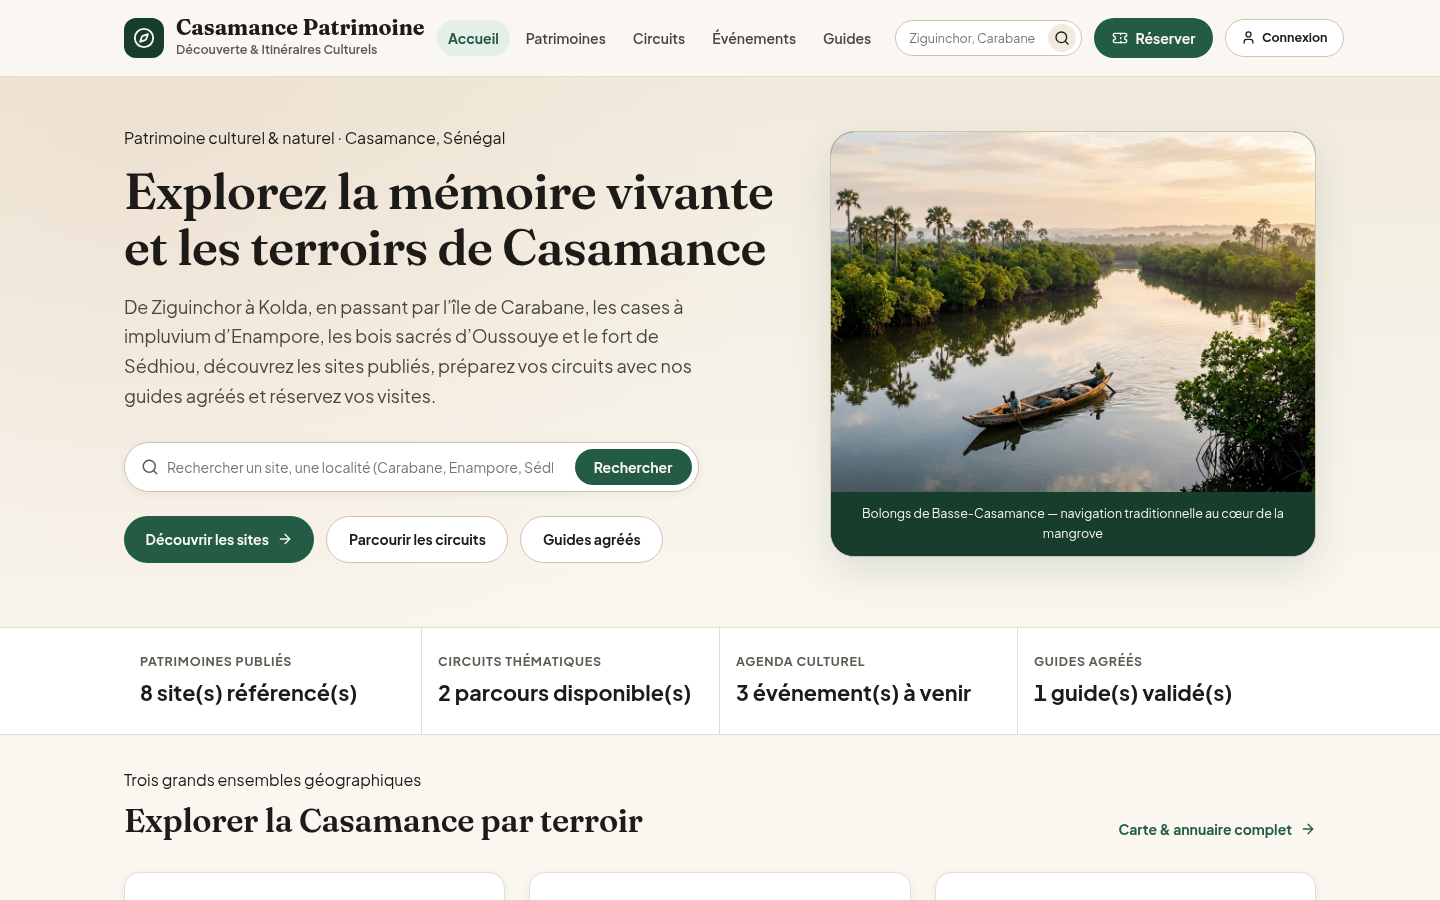
\includegraphics[width=0.92\textwidth]{images/PUB-001_accueil.png}
    \caption{Page d'accueil publique de la plateforme Casamance Patrimoine.}
    \label{fig:pub-accueil}
\end{figure}

\begin{figure}[H]
    \centering
    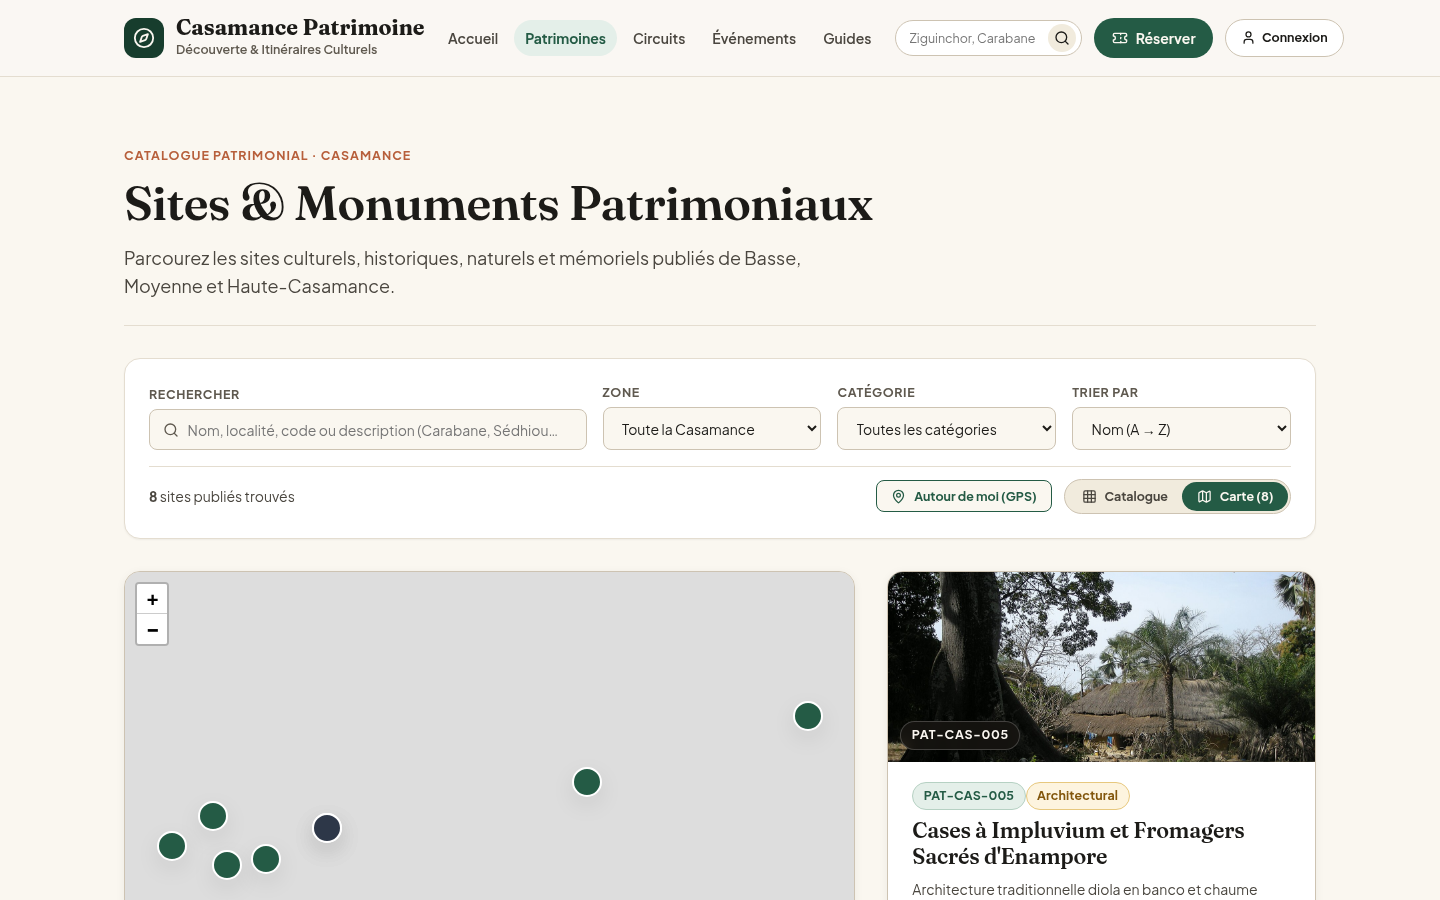
\includegraphics[width=0.92\textwidth]{images/PUB-002_patrimoines-carte.png}
    \caption{Vue cartographique interactive (Leaflet / OpenStreetMap) des sites patrimoniaux.}
    \label{fig:pub-carte}
\end{figure}

\begin{figure}[H]
    \centering
    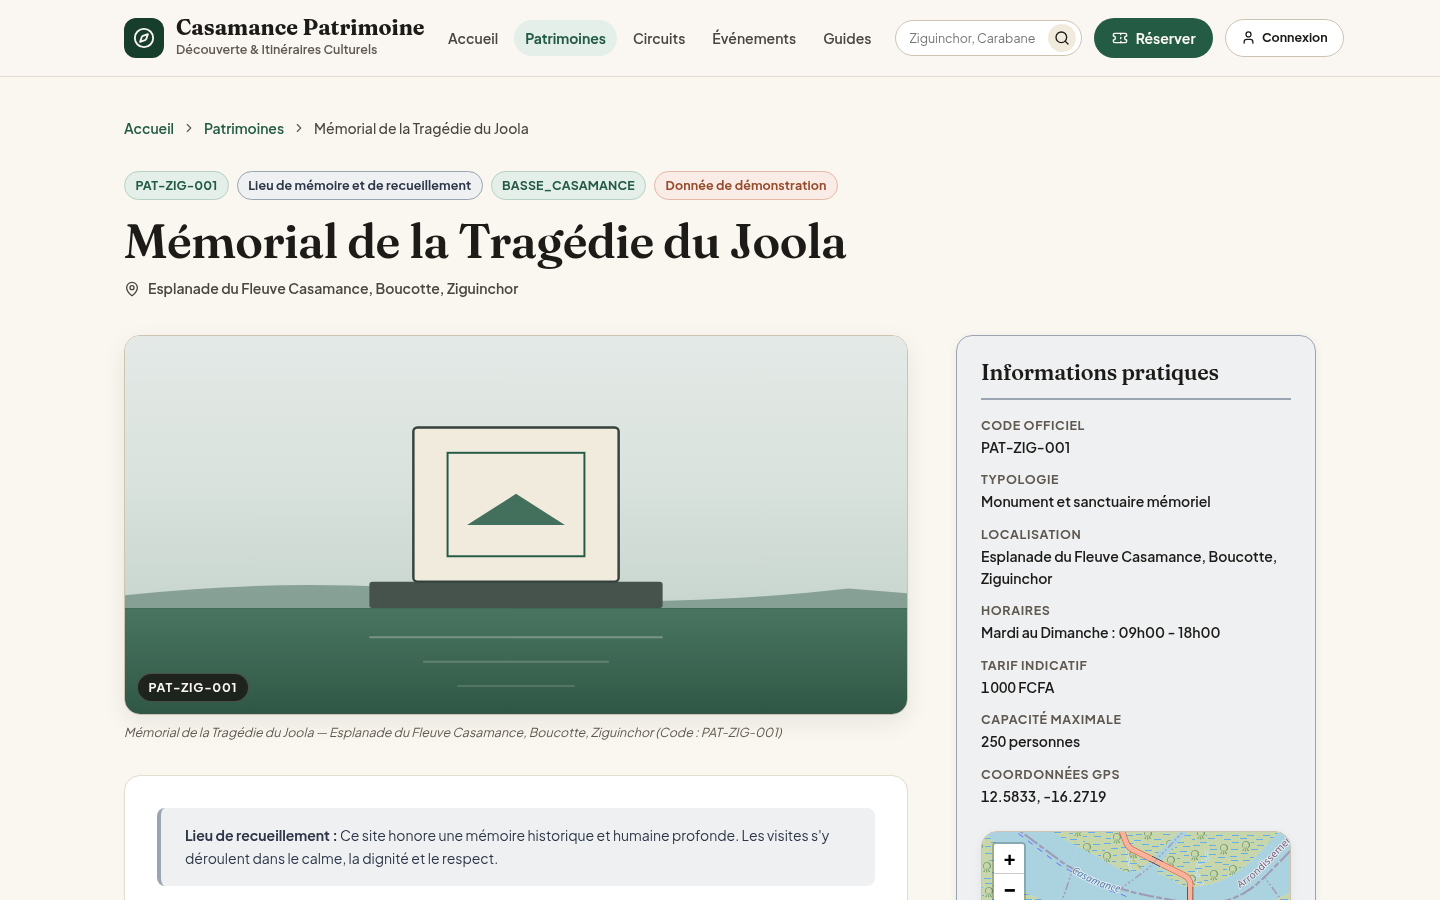
\includegraphics[width=0.92\textwidth]{images/PUB-003_patrimoine-detail.png}
    \caption{Fiche détaillée d'un site patrimonial avec informations géographiques et avis.}
    \label{fig:pub-detail}
\end{figure}

\section{Authentification, Réservation, E-Billet QR et Paiement}
Les touristes disposent d'un parcours complet allant de la connexion sécurisée jusqu'au paiement simulé et à l'obtention d'un billet électronique muni d'un QR Code vérifiable sur site.

\begin{figure}[H]
    \centering
    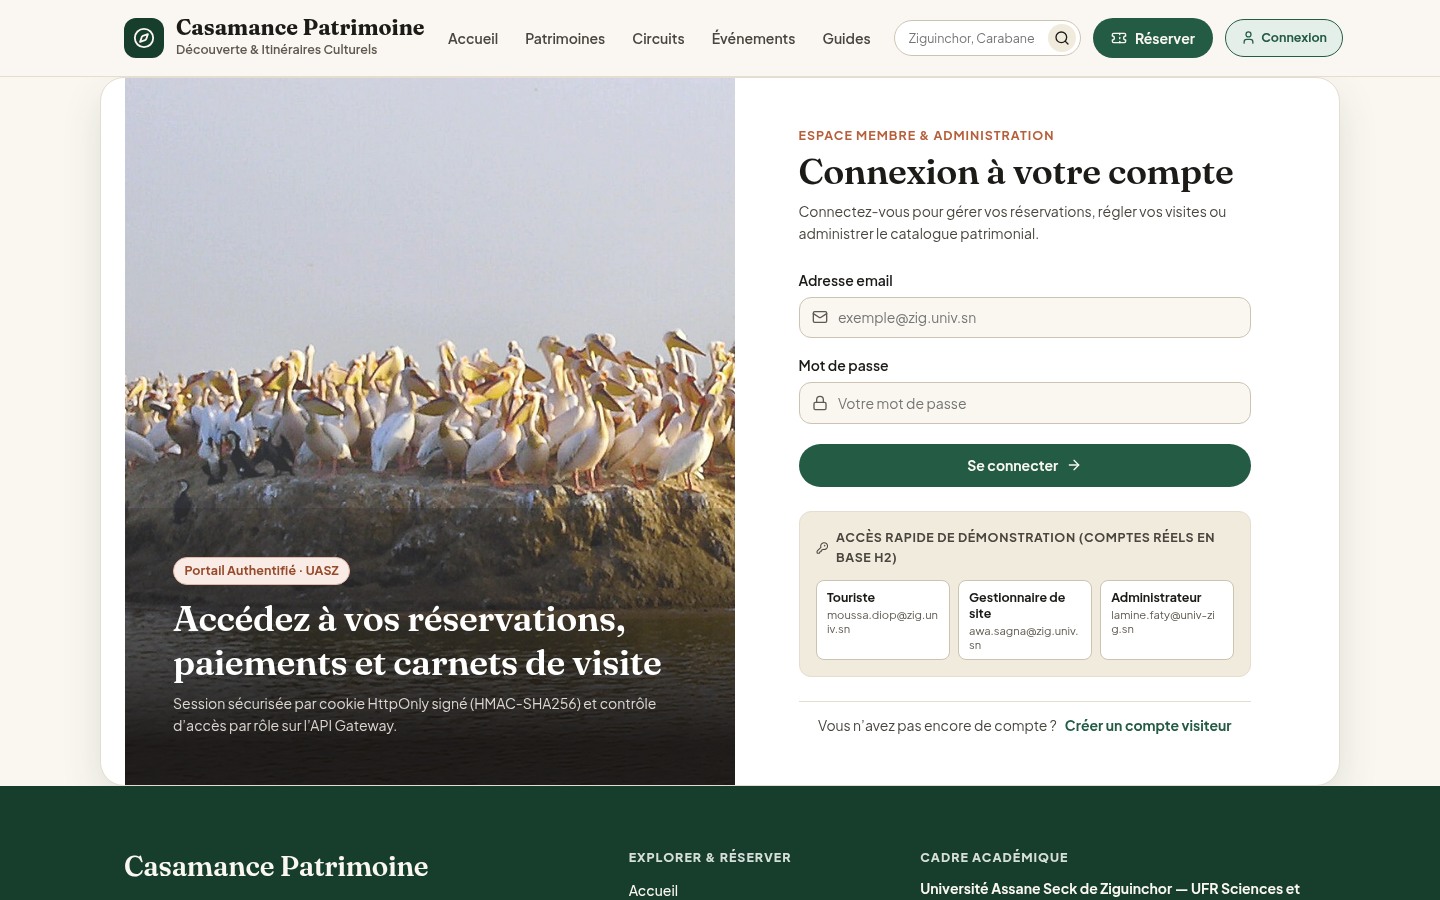
\includegraphics[width=0.88\textwidth]{images/AUTH-001_connexion.png}
    \caption{Interface de connexion sécurisée (session cookie \texttt{HttpOnly}).}
    \label{fig:auth-login}
\end{figure}

\begin{figure}[H]
    \centering
    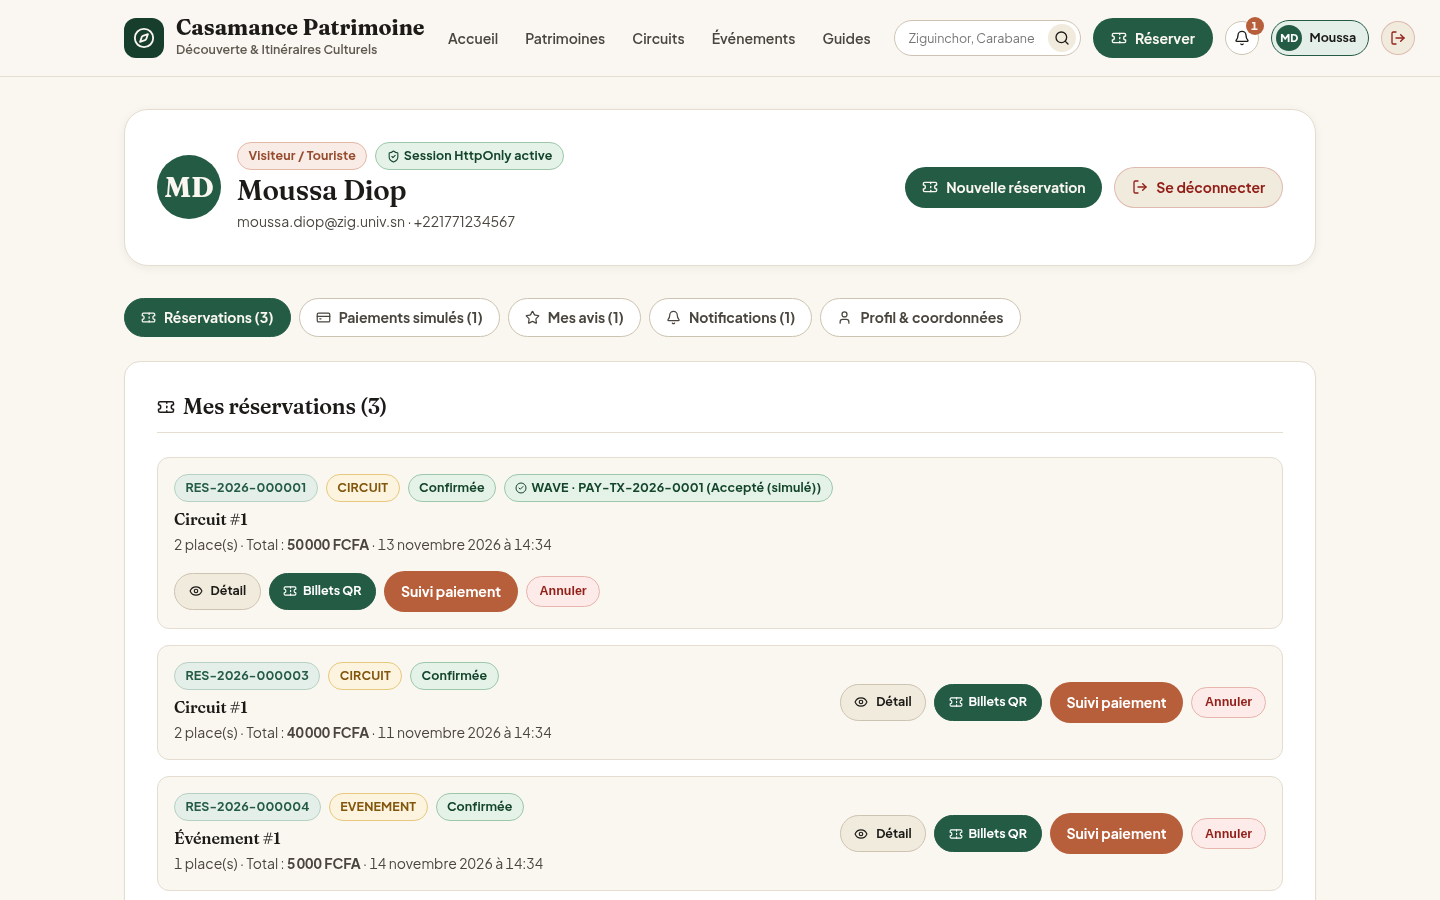
\includegraphics[width=0.92\textwidth]{images/TOUR-001_mon-espace-reservations.png}
    \caption{Espace personnel du touriste : suivi des réservations et statuts.}
    \label{fig:tour-espace}
\end{figure}

\begin{figure}[H]
    \centering
    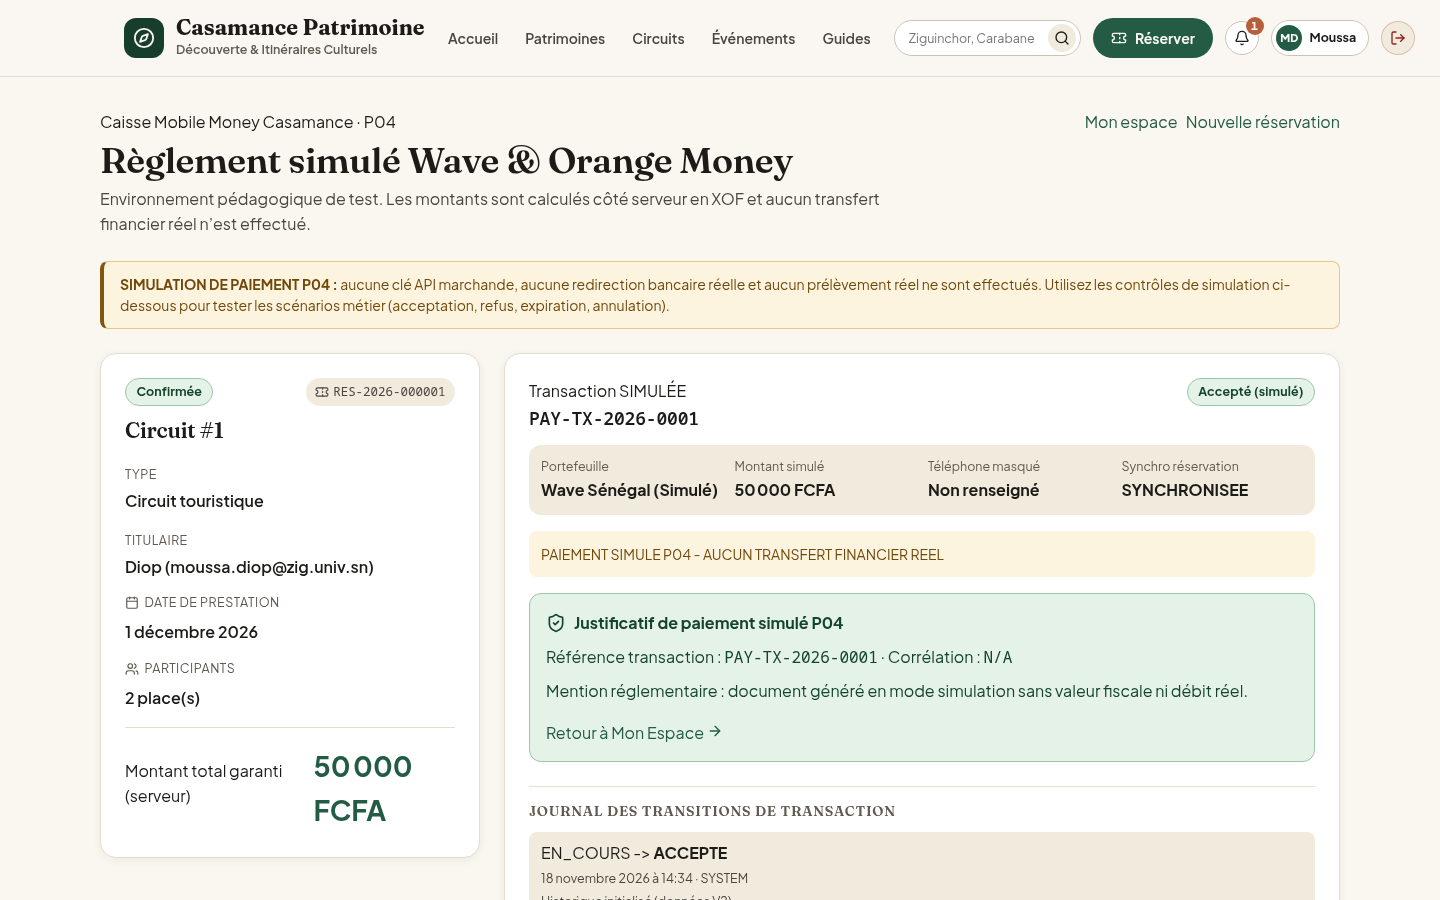
\includegraphics[width=0.92\textwidth]{images/TOUR-004_paiement-checkout-simule.png}
    \caption{Interface de paiement simulé avec gestion d'idempotence.}
    \label{fig:tour-paiement}
\end{figure}

\begin{figure}[H]
    \centering
    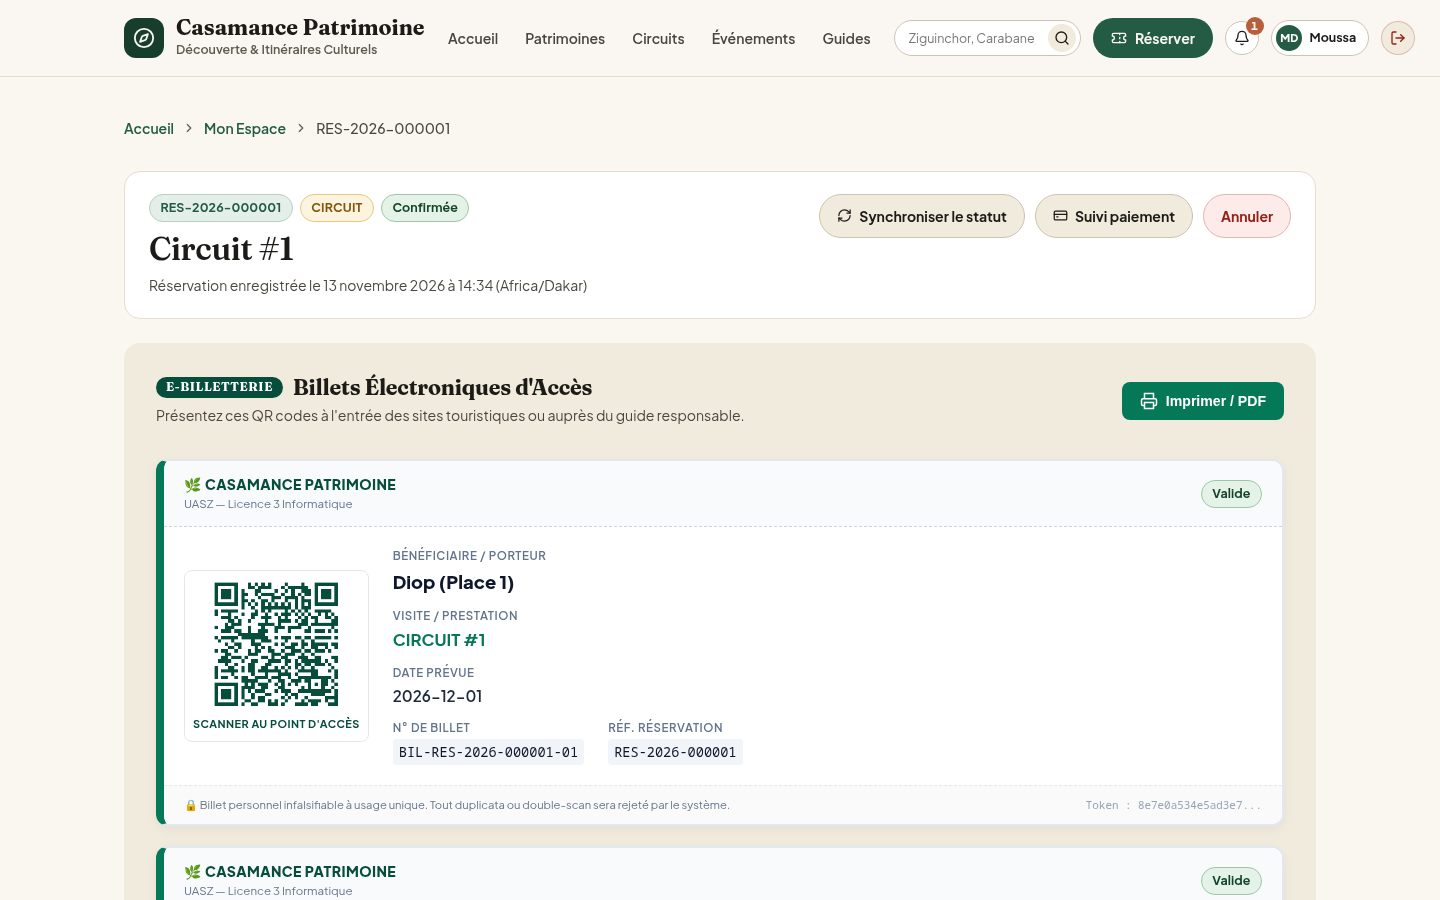
\includegraphics[width=0.92\textwidth]{images/TOUR-003_reservation-detail-qr.png}
    \caption{E-billet électronique avec QR Code généré pour le contrôle d'accès.}
    \label{fig:tour-qr}
\end{figure}

\section{Espaces professionnels et Administration}
Chaque rôle professionnel dispose d'un back-office dédié : tableau de bord Guide, validation des guides par le Conservateur, scanner de contrôle d'accès QR pour les visites, et cockpit d'audit pour l'Administrateur.

\begin{figure}[H]
    \centering
    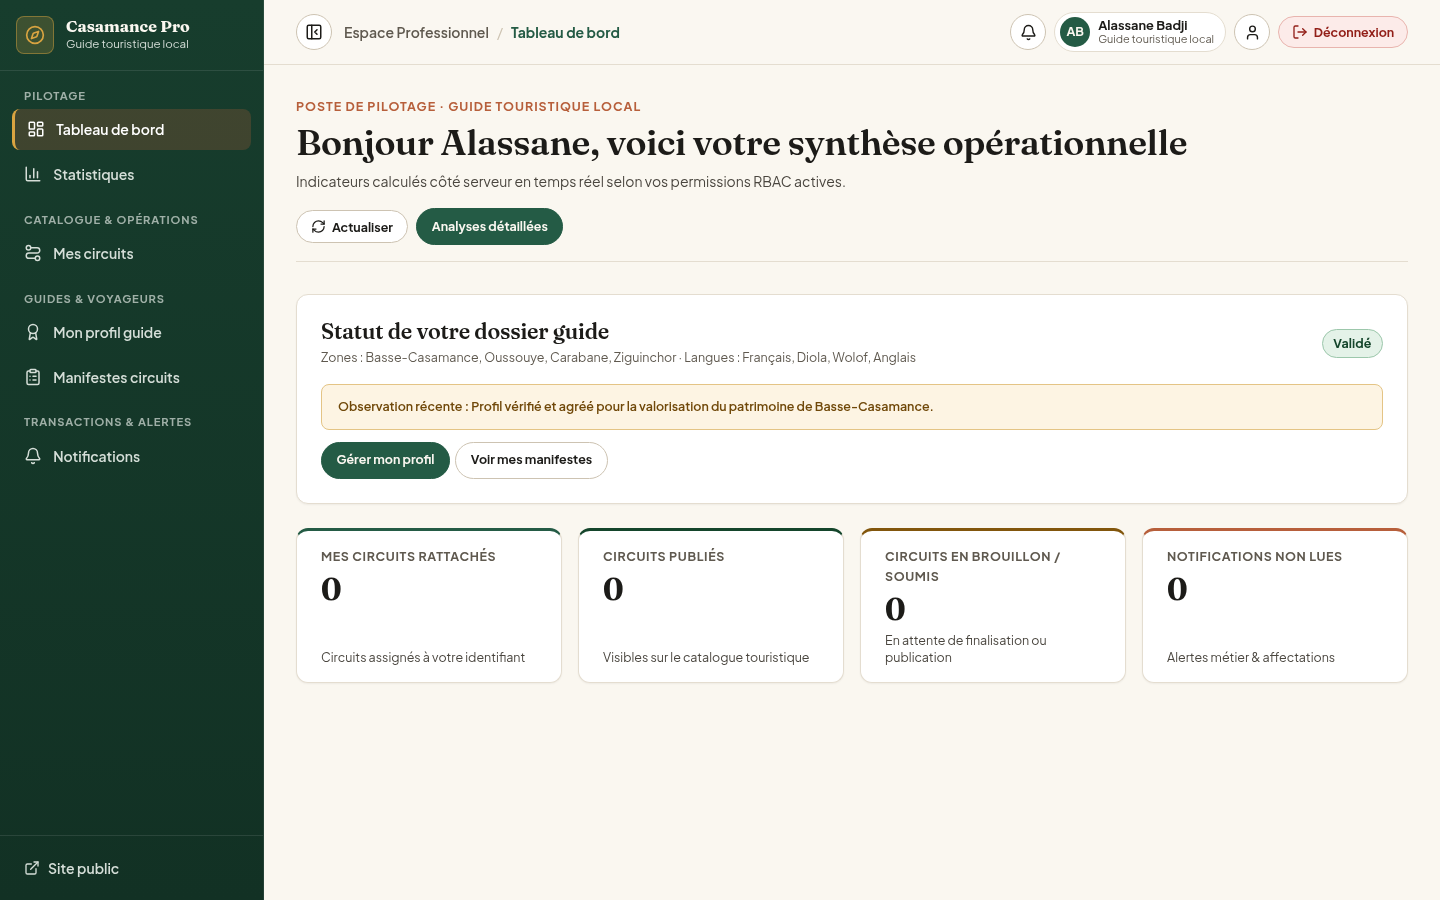
\includegraphics[width=0.92\textwidth]{images/GUIDE-001_tableau-de-bord.png}
    \caption{Tableau de bord du Guide certifié.}
    \label{fig:guide-dash}
\end{figure}

\begin{figure}[H]
    \centering
    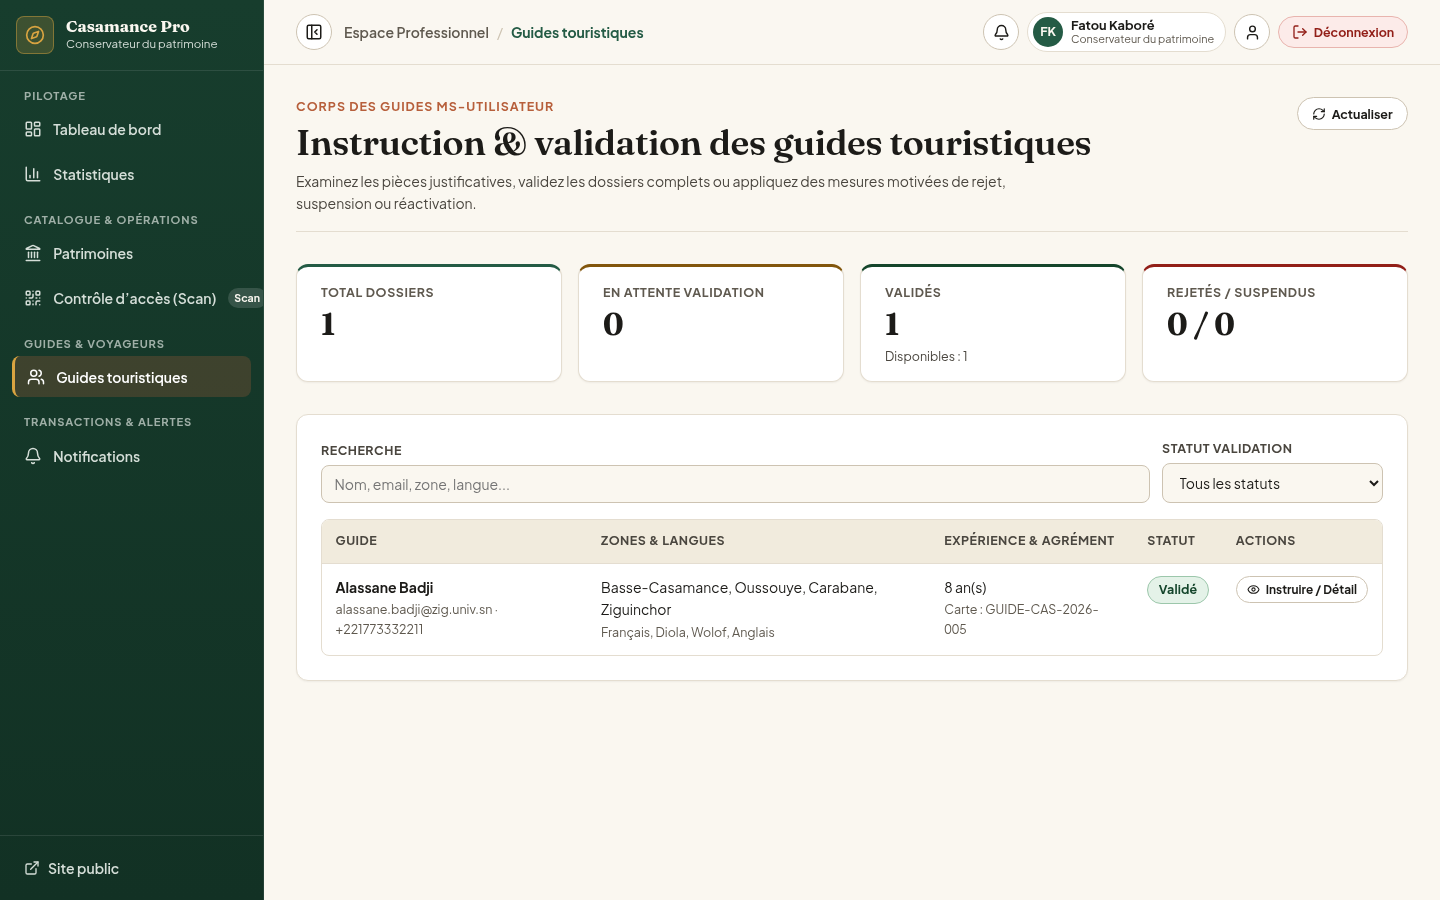
\includegraphics[width=0.92\textwidth]{images/CONS-003_guides-validation.png}
    \caption{Interface Conservateur : validation et suivi des profils guides.}
    \label{fig:cons-guides}
\end{figure}

\begin{figure}[H]
    \centering
    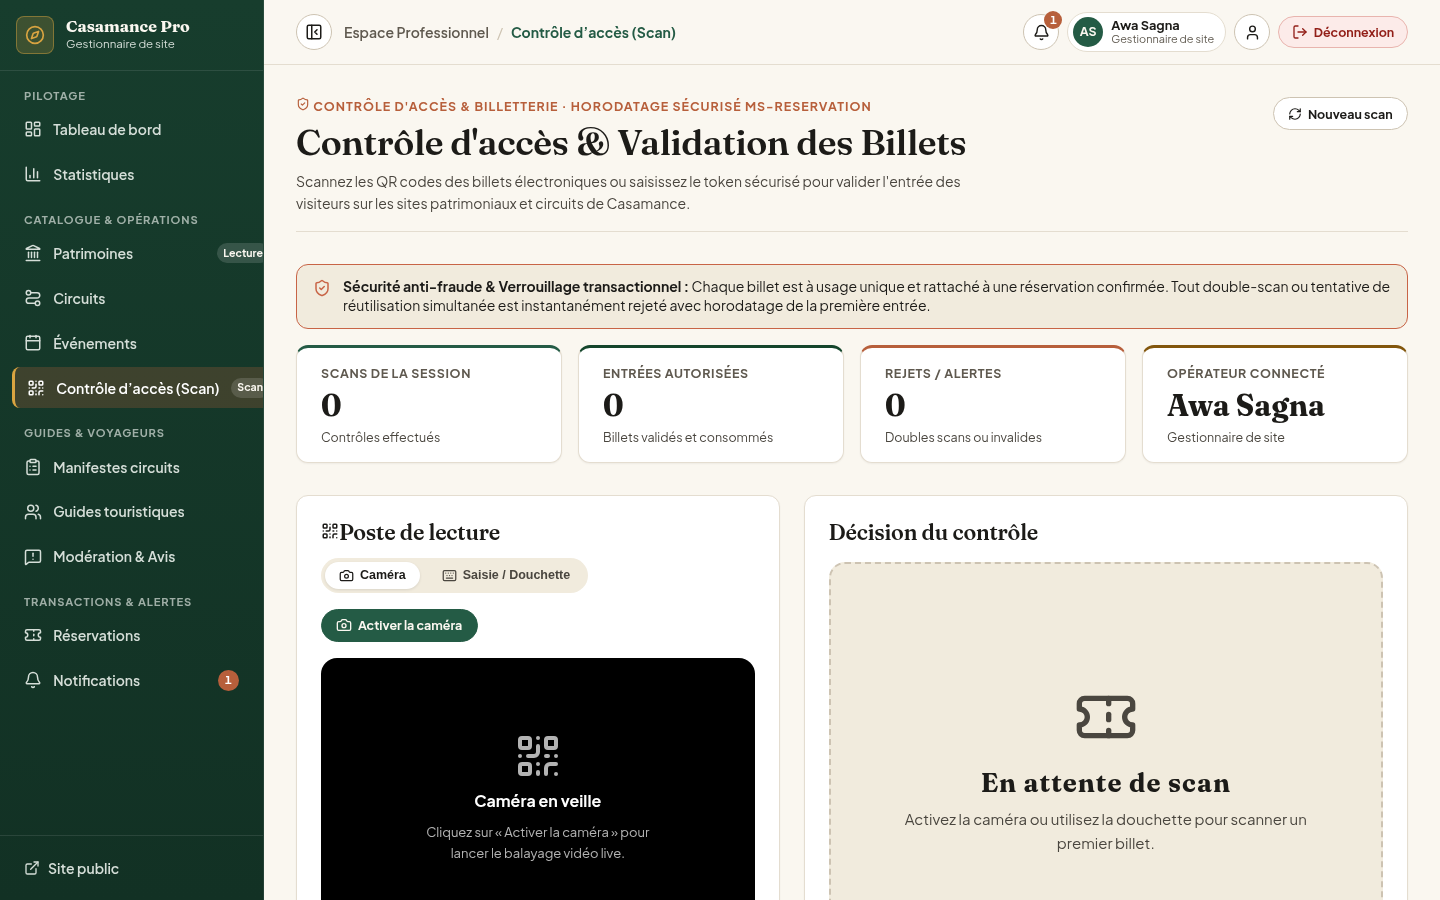
\includegraphics[width=0.92\textwidth]{images/GEST-006_controle-acces-scanner.png}
    \caption{Scanner professionnel de contrôle d'accès des e-billets QR.}
    \label{fig:gest-scanner}
\end{figure}

\begin{figure}[H]
    \centering
    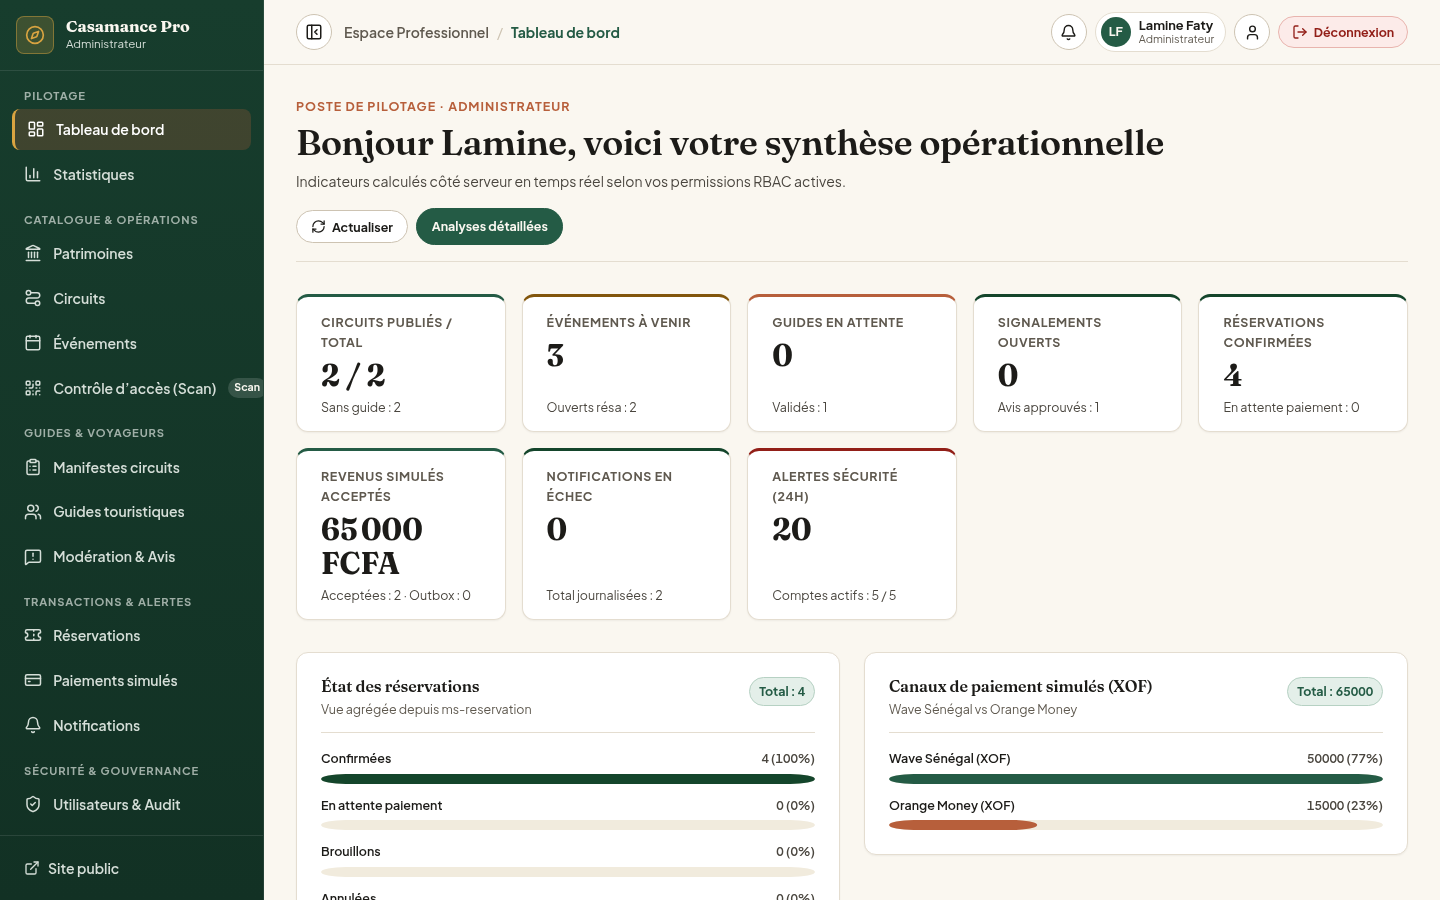
\includegraphics[width=0.92\textwidth]{images/ADMIN-001_cockpit-global.png}
    \caption{Cockpit global d'administration de la plateforme.}
    \label{fig:admin-cockpit}
\end{figure}

\begin{figure}[H]
    \centering
    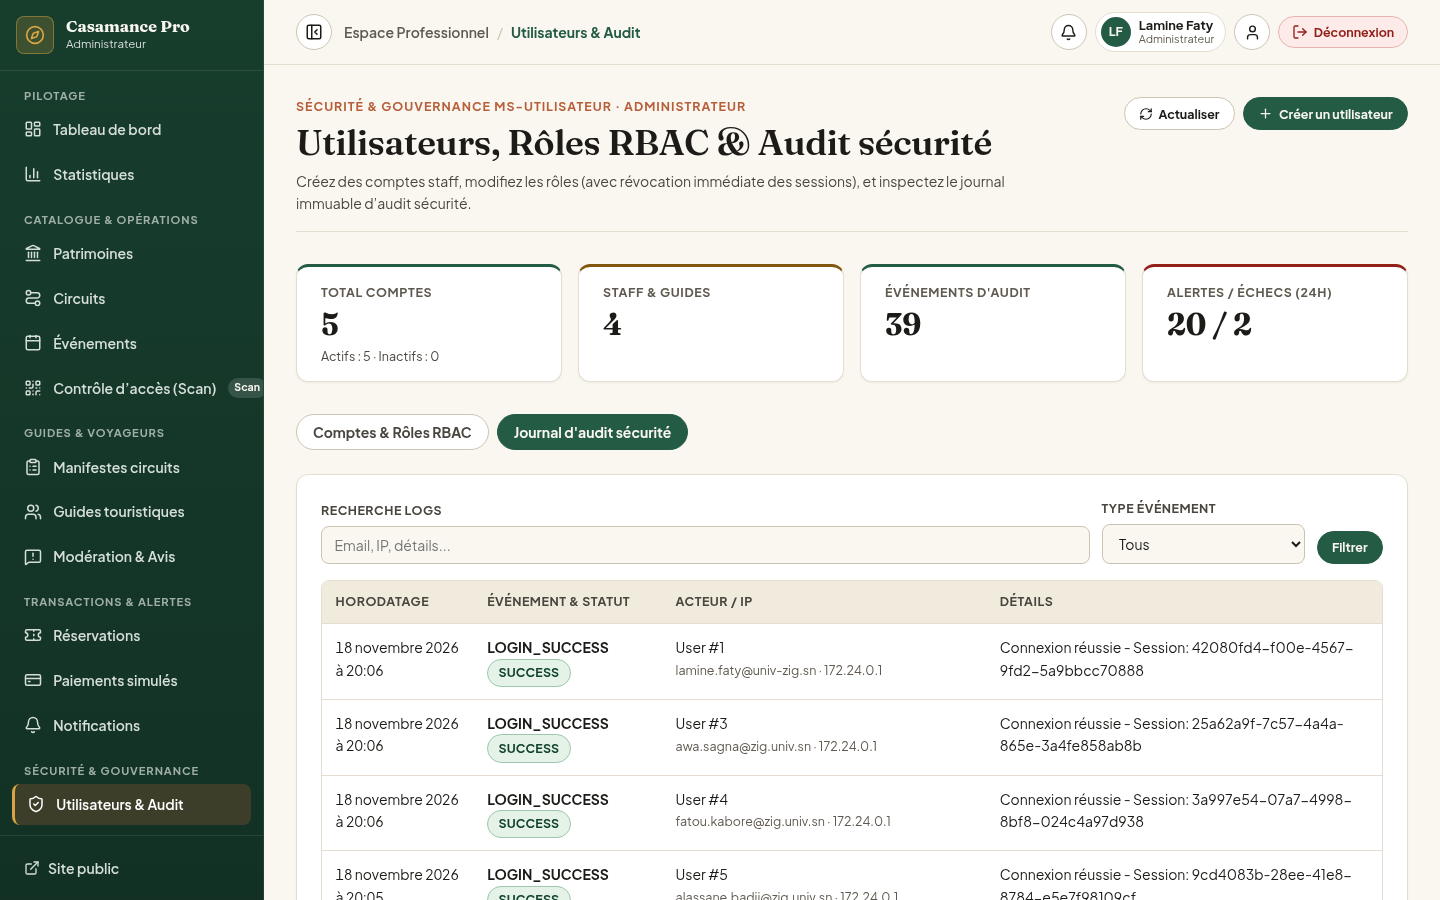
\includegraphics[width=0.92\textwidth]{images/ADMIN-003_audit-securite.png}
    \caption{Journal d'audit de sécurité et supervision des événements critiques.}
    \label{fig:admin-audit}
\end{figure}

% =============================================================================
% CHAPITRE 5 : STRATÉGIE DE TESTS ET VALIDATION
% =============================================================================
\chapter{Stratégie de Tests et Validation Complète}

\section{Tests automatisés Back-End (Maven \& Testcontainers PostgreSQL 16)}
L'exécution complète de \texttt{./mvnw -B clean test} sur les 9 services Java~21 a validé \textbf{214 tests exécutés avec 0 échec et 0 erreur} (dont les tests de concurrence PostgreSQL~16 et d'outbox via Testcontainers).

\begin{table}[H]
\centering
\caption{Résultats des tests unitaires et d'intégration Back-End (9/9 services)}
\label{tab:backend-tests}
\begin{tabular}{@{}l r r r l@{}}
\toprule
\textbf{Service} & \textbf{Exécutés} & \textbf{Échecs / Erreurs} & \textbf{Ignorés (cond.)} & \textbf{Statut} \\
\midrule
\texttt{discovery-server} & 1 & 0 & 0 & \textbf{BUILD SUCCESS} \\
\texttt{ms-patrimoine} & 32 & 0 & 1 & \textbf{BUILD SUCCESS} \\
\texttt{ms-circuit} & 26 & 0 & 2 & \textbf{BUILD SUCCESS} \\
\texttt{ms-evenement} & 19 & 0 & 1 & \textbf{BUILD SUCCESS} \\
\texttt{ms-reservation} & 44 & 0 & 1 & \textbf{BUILD SUCCESS} \\
\texttt{ms-utilisateur} & 36 & 0 & 2 & \textbf{BUILD SUCCESS} \\
\texttt{ms-notification} & 14 & 0 & 1 & \textbf{BUILD SUCCESS} \\
\texttt{ms-paiement} & 16 & 0 & 1 & \textbf{BUILD SUCCESS} \\
\texttt{api-gateway} & 26 & 0 & 0 & \textbf{BUILD SUCCESS} \\
\midrule
\textbf{Total Back-End} & \textbf{214} & \textbf{0} & \textbf{9} & \textbf{9/9 Succès} \\
\bottomrule
\end{tabular}
\end{table}

\section{Tests automatisés Front-End Angular 22 (Vitest)}
L'exécution de \texttt{ng test --no-watch} dans \texttt{frontend-angular/} a validé :
\begin{itemize}
    \item \textbf{26 fichiers de test sur 26 réussis} ;
    \item \textbf{88 tests unitaires sur 88 réussis} (0 échec), couvrant les services API, les composants UI, le lecteur/générateur de QR Code, et les gardes RBAC P06/P07.
\end{itemize}

\section{Validation fonctionnelle en direct dans Google Chrome (\texttt{http://localhost})}
La stack complète (11 conteneurs Docker actifs) a été testée de bout en bout dans Google Chrome :
\begin{itemize}
    \item \textbf{Accueil et catalogue public} : chargement de \texttt{http://localhost/} (HTTP~\texttt{200}), affichage des 8 sites patrimoniaux (\texttt{/api/patrimoines/recherche}~\texttt{200}), fiche détaillée \texttt{/patrimoines/5} avec carte Leaflet, 2 circuits, 3 événements et 1 guide certifié.
    \item \textbf{Parcours d'inscription et session} : création d'un compte touriste (\texttt{POST /api/utilisateurs} $\rightarrow$ HTTP~\texttt{201}), redirection vers \texttt{/mon-espace} avec session \texttt{HttpOnly} active, chargement des réservations, paiements, notifications et avis en HTTP~\texttt{200}.
    \item \textbf{Contrôle d'accès et déconnexion} : accès admin refusé à un touriste (\texttt{GET /api/utilisateurs} $\rightarrow$ HTTP~\texttt{403}), puis déconnexion effective (\texttt{POST /api/utilisateurs/deconnexion} $\rightarrow$ HTTP~\texttt{204}).
\end{itemize}

% =============================================================================
% CHAPITRE 6 : CONCLUSION
% =============================================================================
\chapter{Conclusion}

La plateforme de gestion et de valorisation du patrimoine touristique de la Casamance réalisée par \textbf{Ibrahima DIALLO} et \textbf{Matar NDOUR} sous la direction du \textbf{Dr Lamine FATY} est pleinement opérationnelle, consolidée sur Git et validée à tous les niveaux : architecture microservices, isolation PostgreSQL~16, sécurité Zero-Trust HMAC/RBAC, interface Angular~22 et tests automatisés ainsi qu'en conditions réelles dans Google Chrome.

\end{document}
